\documentclass[12pt]{article}


\usepackage{sbc-template}
\usepackage[utf8]{inputenc}
%\usepackage[brazil]{babel}
\usepackage[hyphens]{url}
\usepackage{hyperref}
\usepackage{graphicx}
\usepackage{caption}
\usepackage{subcaption}


% \usepackage[table,xcdraw]{xcolor}
% \usepackage{caption}
% \usepackage{subcaption}
% \usepackage{booktabs}

\sloppy

\title{Enumeration of operating systems and services in the wireless router's firmware context}

\author{Gianluigi Dal Toso\inst{1}, Lourenço Alves Pereira Júnior\inst{1}}

\address{Divisão de Ciência da Computação\\
  Instituto Tecnológico de Aeronáutica --- ITA\\
  Campo Montenegro -- São Jose dos Campos -- SP -- Brazil
  \email{gianluigi.toso@ga.ita.br,ljr@ita.br}
}

\begin{document} 

\maketitle


\begin{abstract}
The widespread adoption of the home office weakens corporate networks, as it extends its perimeter to homes and ineffective security policies designed for different operating environments. In this context, wireless network routers serve as enablers of access to critical services. However, identifying the software artifacts and possible vulnerabilities present on these devices is challenging, and a heuristic for this purpose is to obtain firmware available on the manufacturers' websites. This paper presents the analysis of $5265$ firmware images downloaded from $5$ vendors' sites, yielding a list of the most common operating systems and services, with the intent of, in a future work, perform security analysis in scale on the obtained firmware images. The exploitation of these components can lead to large-scale attacks, and our results contribute to the vulnerability cataloging process.
\end{abstract}
     
\begin{resumo} 
A ampla adoção do home-office fragiliza as redes corporativas, pois estende seu perímetro até as residências e inefetiva políticas de segurança planejadas para ambientes operacionais diferentes.  Nesse contexto, roteadores de rede sem-fio servem como habilitadores de acesso a serviços críticos.  No entanto, identificar os artefatos de software e possíveis vulnerabilidades presentes nesses equipamentos é desafiador, e uma heurística para esse fim é a obtenção de firmwares disponíveis nos sites dos fabricantes.  Neste artigo apresentamos a análise de $5265$ firmwares e enumeramos os sistemas operacionais e serviços mais comuns, com o intuito de, em trabalho futuro, realizar análises de segurança em escala nos firmwares obtidos. A exploração desses componentes pode culminar em ataques de grande escala, e nossos resultados contribuem para direcionar a catalogação de vulnerabilidades.
\end{resumo}


\section{Introduction}

Cybersecurity is a crucial area in our current context and plays a critical role in the strategic points for business continuity~\cite{wef}. According to the World Economic Forum 2021 Global Risk Report~\cite{wefrep2021}, incidents of this nature represent one of the greatest post-pandemic challenges and have the potential to cause economic disruption, financial losses, geopolitical tensions, and social instabilities. Therefore, it is important to emphasize that cybersecurity should be an essential part of the product and service development lifecycle. It is possible to observe that, in the past, cyber attacks were publicized in specialized media; however, due to the digital transformation the world is undergoing, these types of incidents have appeared in vehicles aimed at the general public (eg, JBS in June 2021\footnote{\url{https://www.nytimes.com/2021 /06/01/business/meat-plant-cyberattack-jbs.html}}, USA Pipelines May 2021\footnote{\url{https://www.bbc.com/news/business-57112371}, \url{http:// /www.nytimes.com/2021/05/10/us/politics/dark-side-hack.html}}, TJ-RS in April 2021\footnote{\url{https://g1.globo.com/ rs/rio-grande-do-sul/noticia/2021/04/29/tj-rs-says-that-court's-computer-system-was-target-of-hacker-attack-and-a lot- grave.ghtml}}, STJ in November 2020\footnote{\url{https://www.cisoadvisor.com.br/stj-comunica-superacao-do-incidente-cibernetico-com-ransomware/}}, just for highlight a few). Hence, there is a relationship between cyber attacks and impacts on different areas of activities in the productive sector~\cite{costs}.

Attacks are not punctually targeted at just a specific system but can be part of large-scale campaigns aimed at orchestrating large-scale malicious activity~\cite{iotbotnet}. In this sense, a typical case deals with compromising computational resources (computers, smartphones, Wi-Fi routers, monitoring cameras, and many other small devices), comprising a command and control chain activated at the attacker's convenience. Internet of Things (IoT) devices are common targets because of their flawed update and maintenance cycle, allowing the creation of botnets like Mirai~\cite{mirai} and Mozi~\cite{mozi}. Therefore, considering the policy of little updating, the neglect of adopting a development process that includes security as an essential element, and the advance in adopting computer systems as enablers of new technological solutions, more and more IoT systems are a frequent target of malicious actors.

Since December of 2019, the COVID's pandemic acts as an unexpected groundbreaking factor that changed humanity's course.  The ability to work in a person's home has been an increasing desire in society, and following the fast advances in technology, companies were already experimenting with remote models of work. However, amidst the COVID-19 pandemic, many cities imposed mobility restrictions in order to restrain virus spreading.  As companies have adopted remote work, there is a tendency to increase this model considerably in a post-COVID world.  Working from home expands the companies' network perimeter, exposing digital assets to new threats and vulnerabilities. Consequently, it causes an increase in a company's attack surface as small and home office types of equipment are potentially more vulnerable. Home wireless routers, for instance, are the worker's first access to the internet and may be running firmware with security breaches that could leverage to provoke a cybersecurity incident~\cite{soho}.

Identifying the software artifacts present on these devices is challenging due to the wide adoption of these devices in the small and home-office (SOHO) context and requires a considerable amount of computational effort to infer. Therefore, a heuristic approach is convenient to succeed in such a task, providing the infeasibility to perform reconnaissance on a large scale. One approach is to detect vulnerabilities in firmware products before the attackers and report them back to the vendor to prevent this kind of attack. Once determined, the manufactures can patch the system to fix the identified security breaches and release the binary in their sites.  Furthermore, a heuristic for this purpose is to obtain firmware available on the vendors' websites.  
% falar sobre re-hosting
% falar sobre os resultados obtidos
% 
This paper aims to discuss a way to automate the security analysis and vulnerability detection in wireless router firmware via re-hosting the original firmware in an emulator before executing vulnerability analysis and discovery techniques.  We present the enumeration of $5265$ downloaded from $5$ vendors' sites, yielding a list of the most common operating systems and services. The pieces of information gathered in this enumeration can be used to determine the most prominent target for exploitation. Firmware images matching this target can then be scanned for vulnerabilities. One way to search for vulnerabilities in scale is to re-host the target firmware images in an emulator so that it can execute without the real device, and using vulnerability detection techniques, such as fuzzing, against the re-hosted firmware. The exploitation of these components can lead to large-scale attacks, and our results contribute to the vulnerability cataloging process.

With this work. we aim to prevent future network router attacks by assuming the attacker position in enumerating the most common resources and vulnerabilities found in network devices firmware images. Our intention is to investigate if from the large amount of firmware available from open sources (vendors' sites), it could be possible to extract enough knowledge so that a large scale attack could be performed. If that is the case, vendors could be warned, allowing them to patch their devices.

This paper's remainder is structured as follows. We describe the most relevant related solutions in Section~\ref{sec:related}.  In Section~\ref{sec:methodology}, we describe our approach to perform wireless router reconnaissance. We describe the validation of our proposal and the results in Section~\ref{sec:results}. Finally, we summarize our work and provide future works in Section~\ref{sec:conclusions}.


\section{Related Works}
\label{sec:related}

Considering the context of our study, understand the running components (operating systems, file systems, services) in the router's firmware contribute to the re-hosting.  Re-hosting is a technique for executing a tightly coupled system in another hardware or platform (in our case, in emulation).  Thus, our contribution relies upon this context.  We observed different approaches regarding overcoming re-hosting difficulties caused by the need for peripherals of the original hardware that are not present in the emulated device. For example, the work of \cite{firmware-challenges} surveys the prominent techniques used in firmware re-hosting to bypass actual hardware dependency. Thereby, the four most common approaches are Partial Emulation, Fuzzing, Learning, and Abstraction Replacement.

\subsection{Partial Emulation}

Partial emulation, also known as ``hardware in the loop'', consists of emulating most firmware execution; however, redirecting to the actual device hardware calls when the firmware asks for a peripheral is infeasible. This approach requires having an actual device available, and for this reason, it does not scale. Execution fidelity, on the other hand, is pretty close to the actual hardware execution. The work of \cite{surrogates} enhances hardware redirecting by building a hardware bridge using an FPGA board to connect the PCI bus on the emulating host with the PCI bus on the actual embedded device, an approach they called {\tt SURROGATES}.

The work of \cite{avatar2} extensively explores vulnerability discovery in embedded devices using the hardware in the loop technique. They use a symbolic engine builds upon QEMU called {\tt S2E} to search for vulnerabilities in IoT devices through re-hosting and to redirect peripherals calls to the actual hardware. In addition, they implement a tool called {\tt Avatar$^2$} as a reverse engineering framework based on the hardware in the loop approach.  Nonetheless, the dependency on the physical systems imposes barriers in testing.

\subsection{Fuzzing}

To overcome the partial emulating techniques, Fuzzing is a re-hosting approach to hardware dependence (not to be confused with fuzzing as a vulnerability discovery technique) because hardware calls to peripherals do not need the peripheral to be successful. Instead, the actual peripheral response request to the hardware call is just a binary value. Therefore, knowing the range of values that provide an acceptable answer to the hardware call, selecting any random value within this range is enough to keep executing the emulated system.

\cite{p2im} effectively implements this kind of hardware bypass.  The authors present an approach to model the interface between the processor and the peripheral. The method suggested is called {\tt P2IM} - Processor-Peripheral Interface Modeling.  However, it requires a human specialist to model the interface between the CPU and a specific peripheral to determine the specific range of values to each hardware call. Therefore, this approach also does not provide a scalable solution, requiring human intervention (to model the interface).

\subsection{Learning}

Learning is a similar approach to fuzzing for re-hosting, as it relies on the fact that to bypass hardware dependence, it is only needed to return expected values to hardware calls. However, the learning approach, as used in \cite{pretender} first monitors actual hardware execution and registers each hardware-peripheral interaction. Then it uses a Machine Learning algorithm to build a model of the interface (in contrast to using a human specialist as in the fuzzing approach). As a result, the learning technique produces a better interface to simulate peripheral interaction; however, it also depends on having the actual hardware first to build the interface's working model, which impedes its scalability.

\subsection{Abstraction Replacement}

Abstraction Replacement takes a different approach, and instead of producing answers to hardware calls that are similar to the responses real hardware would produce, this method tries to remove from the original firmware the hardware call, replacing it with another abstraction not requiring the actual hardware.

In the work of \cite{halucinator}, they develop the method called {\tt Halucinator}, whose idea is to search for Hardware Abstraction Layer (HAL) libraries inside the firmware and replace those libraries with custom libraries implemented by the researchers that do not require peripherals to work. However, this method still requires human intervention for each firmware and thus, still does not scale.

On the other hand, the work of \cite{firmadyne} implements a tool called {\tt Firmadyne}, whose approach to re-hosting consists of replacing the original kernel found on the firmware image with a custom implemented and instrumented kernel worked by their team (the same kernel is used to all firmware images emulated, regardless their original kernel version). This approach allows firmware emulation to be done at scale, with the counterpart that the kernel replacement sacrifices emulation fidelity. The authors of {\tt Firmadyne} also implemented a web scraper capable of downloading firmware binary from popular vendors website and then used {\tt Firmadyne} to emulate and perform security analysis on the downloaded firmware images. % A forked version of the web scraper developed with {\tt Firmadyne} was used in our research to acquire firmware images from network routers vendors' websites.

%They can then emulate firmware at scale, with the counterpart that the kernel replacement sacrifices emulation fidelity.

\subsection{Summary}

As we can see, many of the re-hosting techniques rely on non-scalable mechanisms. For example, Hallucinator and Firmadyne provide an improvement to enable analysis at scale; however, they impose limitations and remove much software running in kernel mode.  We present a proposal that differs from others by increasing the re-hosting coverage of operating systems in small and home-office systems (SOHO).  Our work provides a vision of operating systems to focus on, including a hardware architecture, version, and file systems.  Hence, identify dependencies in components (specific drivers) and maximize artifacts with favorable prominence (e.g., network stack).  As a result, it advances the state-of-the-art by bringing pieces of software left out of the emulation loop.

\section{SCREEN: {\bf S}craper, {\bf C}lustering, {\bf RE}-hosting, and {\bf E}xploitatio{\bf N}}
\label{sec:methodology}

This section presents an architecture for examining firmware available for download on vendors' websites to discover the most common components. Next, we focus on pieces of software (or artifacts) targeted to run in kernel mode.  Hence, we define SCREEN: {\bf S}craper, {\bf C}lustering, {\bf RE}-hosting, and {\bf E}xploitatio{\bf N}.  Our research enables the evaluation of SOHO in the large-scale re-hosting of router firmware images based on Linux kernel and the innovative aspects of the approach intended in this project.


\subsection{The Architecture description}
This paper represents only part of a solution idealized for a more extensive research project to be conducted throughout the years by a team of researchers. Figure \ref{fig:architecture} illustrates the overview of the architecture for the complete project, whereas in this paper, we focus on the re-hosting part of the proposed architecture.

\begin{figure}[h]
    \centering
    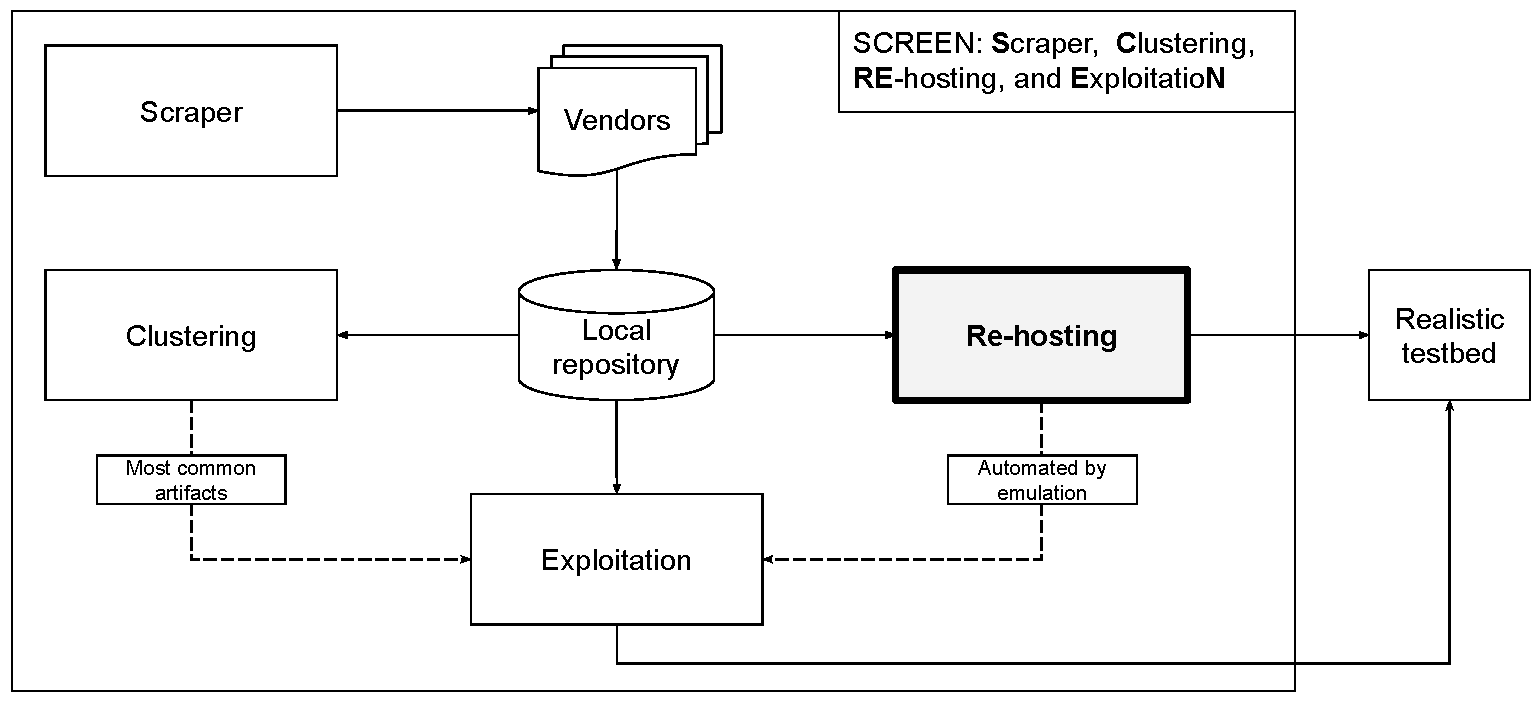
\includegraphics[width=\textwidth]{sebseg/screen}
    \caption{Architecture proposed for a complete solution in firmware vulnerability analysis.}
    \label{fig:architecture}
\end{figure}

The complete architecture includes a scraper module consisting of a web crawler responsible for entering router vendors' websites and downloading for a local repository the most considerable amount of firmware images available as possible. The re-hosting experiments require the availability of firmware images. In this stage, the scraper module serve the purpose of providing a minimum amount of firmware images to allow the research in the re-hosting process. Therefore, we adopt Firmadyne's \cite{firmadyne} as baseline to implement our scraper.  Our project is expanding the Firmadyne's scraper by adding more vendors to the list, as we are adding new sources to it.

From the local repository, two different modules perform actions using the acquired firmware. First, the re-hosting module is responsible for extracting firmware images (and collecting information about the firmware in the process) and preparing the firmware image to be emulated. As this module is the focus of this paper, Section \ref{sec:re-hosting} will explain this process in detail. The other module to perform actions in firmware images contained in the local repository is the clustering module. It consists of searching for similarities and patterns amongst different firmware images. The results obtained by the clustering modules are helpful in steps to improve the vulnerability analysis and discovery process.

Finally, the exploitation module provides means to create weapons to abuse the targeted systems. In this stage, vulnerability analysis (using frameworks to detect known software vulnerabilities) and vulnerability discovery (such as fuzzing techniques) is applied to the emulated firmware to analyze its security performance.

\subsection{Firmware Extraction}
\label{sec:extraction}

For the firmware extraction process, our research focuses on enhancing the original script provided with Firmadyne for firmware extraction developed in Python and making extensive use of {\tt binwalk}'s API. This original script uses {\tt binwalk} to recursively extract the firmware image setting a limit for depth and breadth in order to limit this process as it is prolonged. Furthermore, to speed up the extraction, the {\tt /tmp} directory of the host system (which stores files during the firmware extraction process temporarily) is going to be mounted on the {\tt tmpfs} provided by the Linux kernel, and that allows us to mount a directory in the RAM instead of mounting it on the disk.

Nonetheless, this method is potentially incapable of automatically extract some firmware images. Because not all firmware follows standard implementation, and frequently vendors obfuscate compression and file systems, we marked the failure subjects to posterior examination. Afterward, we inspect the marked ones to identify constraints and verify how to improve the automated image extraction. Then, subsequent modifying the extraction script, this entire process is repeated until satisfactory reach the maximum level in the extracted firmware images.

\subsection{Re-hosting Process}
\label{sec:re-hosting}

We aim to maximize the portion of the original firmware during the re-hosting phase, absenting the original hardware. Firmadyne's approach to firmware re-hosting extracts from the original firmware image its original root filesystem and kernel. It then completely ignores the original kernel and replaces it with a custom instrumented kernel designed by the researchers (they developed one instrumented kernel for {\tt ARM} architecture and one for {\tt MIPS} architecture). Finally, the {\tt QEMU} tool is responsible for the emulation process, which uses binary translation to allow the execution of binaries from different architectures. The emulated firmware is emulated with {\tt QEMU} using the instrumented kernel together with the extracted filesystem from the original firmware.

Our approach to firmware re-hosting is similar to Firmadyne's one, with differences regarding the kernel replacement part. Instead of just building one heavily instrumented kernel and replacing all firmware images with that same instrumented kernel, we propose building-specific kernel versions on demand according to the original kernel used by the firmware image under emulation. With that, our heuristics correspond to use a more similar kernel to the original to reduce incompatibility with network drivers and modules and therefore increase the number of emulated firmware with a working network interface. In addition, increasing the emulation coverage allow us to extend the vulnerability analysis and discovery process to a more significant amount of router firmware images than the one covered by the original Firmadyne's implementation.

This process of automated kernel cross-compilation, however, faces many issues. The first one is how to define a valid kernel compile configuration that results in a kernel that has the features expected in router firmware. Kernel compile configuration is a configuration file ({\tt .config}) where the user can configure an extensive list of parameters to include or exclude features to the compiled kernel.

These configuration files can be filled up by the user manually, via answering questions interactively in the command-line interface, or ultimately adopting an existing file used by a current firmware's kernel previously compiled. Defining how to produce a good {\tt .config} file is already an open problem in our research. Another idea is to extract kernel compilation default configuration from OpenWrt Linux systems. The OpenWrt is a Linux targeted to serve as an open-firmware for wireless routers. Thereby, OpenWrt images may have kernel configurations compatible with most networking features expected from a wireless router. In this way, in this research, we plan to investigate the better way to produce a valid compilation configuration file to allow kernel compiling.

After choosing a valid kernel compilation configuration file, the kernel has to be cross-compiled in the host machine to compile for the architecture expected in the original firmware image. Unfortunately, kernel cross-compilation is also challenging, as the compilation process is heavily dependent on its toolchain (compiler, utilities, and libraries versions). Furthermore, it means that to compile multiple different kernel versions automatically; there must be a way to automatically switch between a set of known working toolchains for each kernel version.

Another approach, to reduce the number of parameters that need to be configured in order to build a very tailored kernel for each firmware, could be to use the enumeration and focus on building a repository with the most common kernel versions (or at least kernel families). Then, for the re-hosting, for each firmware image, an heuristic could be used to determine which compiled kernel from the repository is the most similar to the original kernel expected from the firmware. This matching kernel could then be selected to be used during the re-hosting process.

After compiling a kernel version that matches the original kernel, the firmware image is then ready to be emulated using the {\tt QEMU}. First, the newly compiled kernel serves as firmware in emulation with the original filesystem extracted from the firmware sample. After that, following the work of \cite{firmadyne}, we evaluate if these emulated firmware images can infer and configure the network successfully. If that is the case, vulnerability analysis and discovery techniques are applied (using standard tools for this purpose). Finally, the results obtained are helpful to evaluate overall firmware security, reporting the mapped vulnerable products (if that happens) to the vendor.

Figure \ref{fig:firmadyne-screen-compare} illustrates how the SCREEN approach to re-hosting differs from the one used by Firmadyne. While Firmadyne uses one heavily instrumented kernel with all firmware images during the re-hosting process, SCREEN will build kernels using the information gathered from the firmware images and select a more suitable kernel from the repository to use when re-hosting a specific firmware image.

\begin{figure}[h]
     \centering
     \begin{subfigure}[b]{0.45\textwidth}
         \centering
         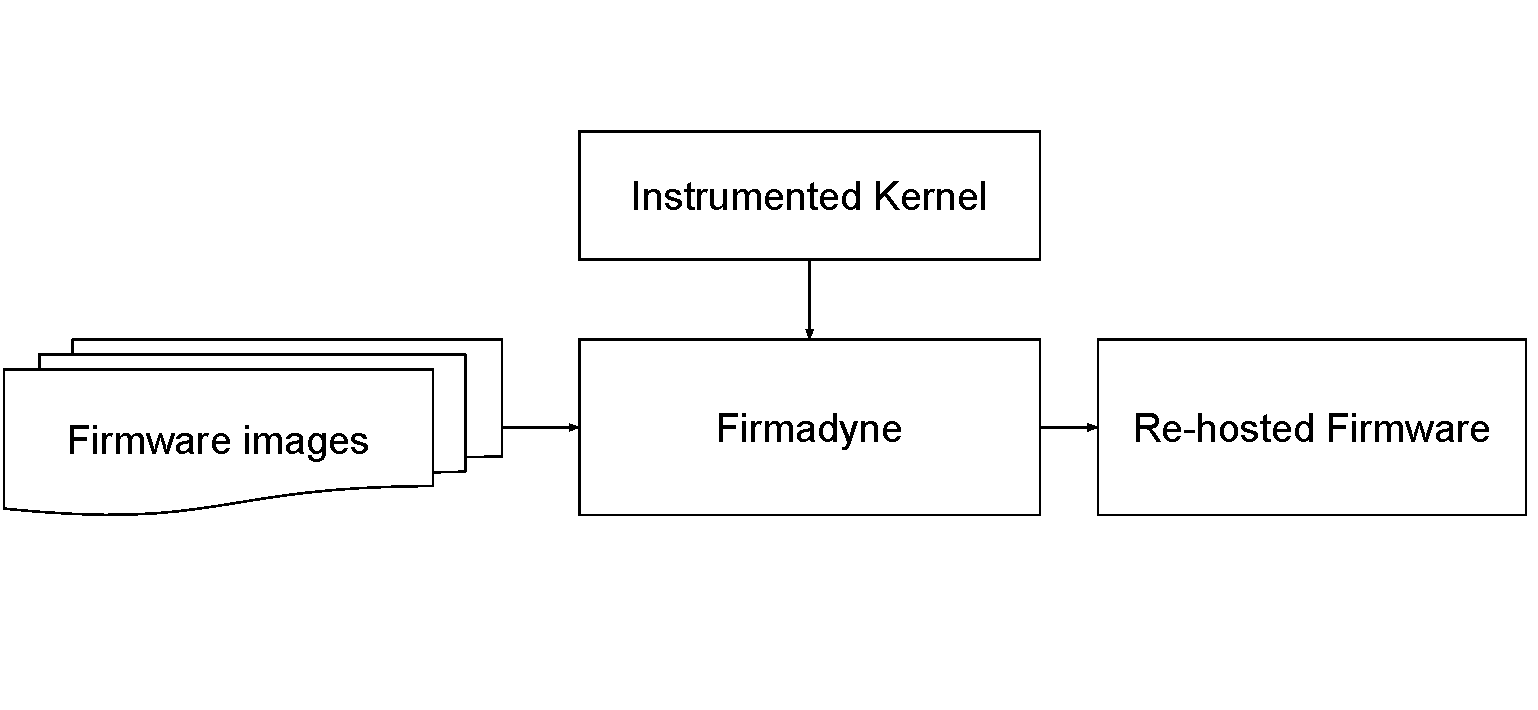
\includegraphics[width=\textwidth]{sebseg/Firmadyne-Approach.pdf}
         \caption{Firmadyne approach to re-hosting.}
         \label{fig:firmadyne-approach}
     \end{subfigure}
     \hfill
     \begin{subfigure}[b]{0.45\textwidth}
         \centering
         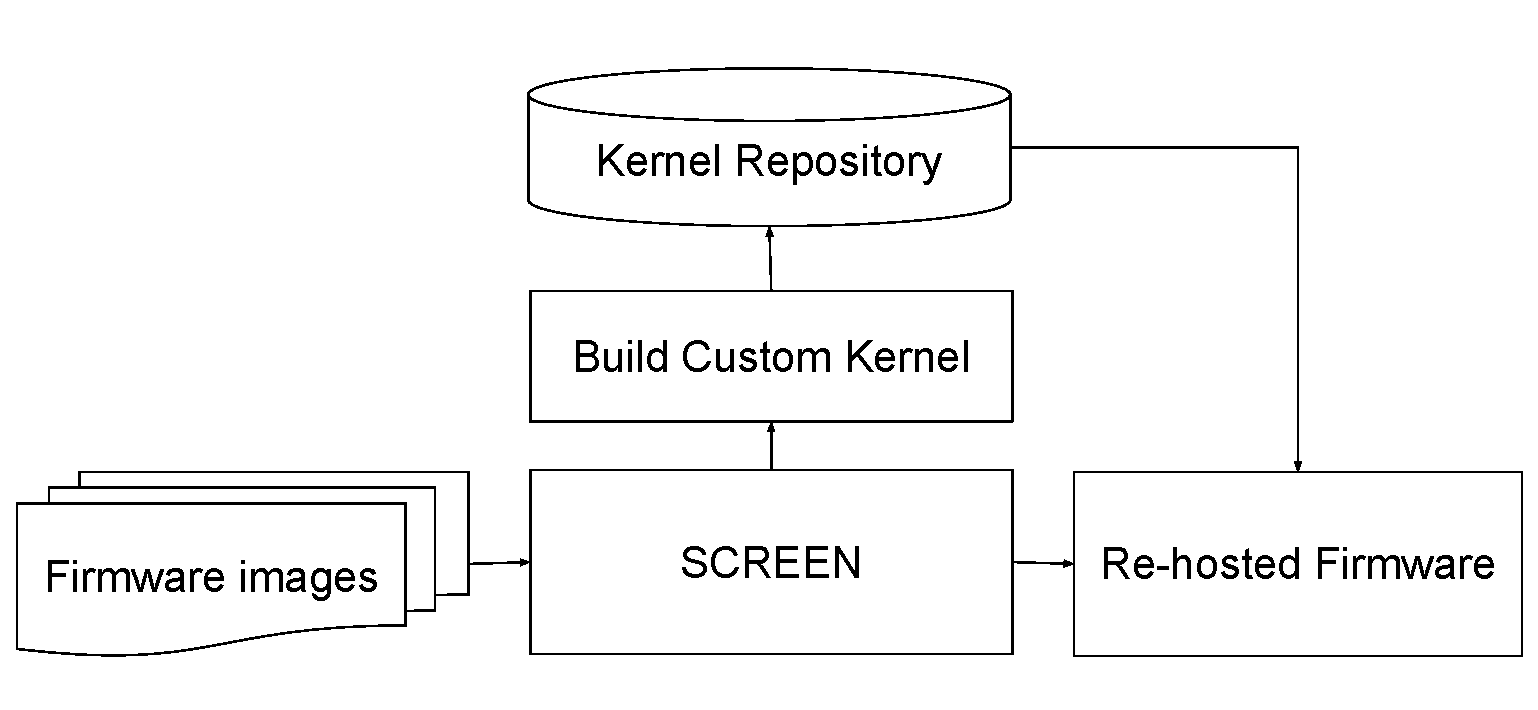
\includegraphics[width=\textwidth]{sebseg/SCREEN-Approach.pdf}
         \caption{SCREEN approach to re-hosting.}
         \label{fig:screen-approach}
     \end{subfigure}
        \caption{Comparison between the approaches used by Firmadyne and SCREEN during the re-hosting phase.}
        \label{fig:firmadyne-screen-compare}
\end{figure}

\section{Results}
\label{sec:results}

When considering the analysis on a large scale, one can experience a wide range of heterogeneity in firmware components and operating systems.  Pragmatically, a full re-hosting by emulation is impossible by nature; then, discover the most common artifacts is crucial to steer efforts on porting components to QEMU.  In this Section, we realize the first step in the SCREEN re-hosting phase by identifying operating systems, architecture, and file systems. Then, we discuss the results obtained in firmware acquisition and firmware extraction. We improve Firmadyne performance (our baseline), serving as a demonstration of our approach.


\subsection{Firmware acquisition}

For the firmware acquisition, we used a fork of the Firmadyne's original scraper \cite{github:scraper}. This modified scraper version has fixed some compatibility issues the original scraper has with Python 3 and also updates the spiders to match the more updated version of vendor websites. Without modifying any of the spiders provided by the scraper, we selected five vendors (these five vendors were selected at random, as a mean to start the research, but the final goal is to use all available vendors within the scraper) and executed the scraper to find and download firmware from these vendors' websites automatically. In total, we downloaded 5265 firmware images throughout this process. Table \ref{tab:scraper} shows the number of firmware images and its combined file size for each vendor.

\begin{table}[h]
\centering
\caption{Downloaded firmware images per vendor}
\begin{tabular}{|c|c|c|}
\hline
\textbf{Vendor} & \textbf{Firmware Images} & \textbf{Combined File Size} \\ \hline
Netgear         & 3122                     & 93 GB                       \\ \hline
TP-Link         & 1320                     & 10 GB                       \\ \hline
D-Link          & 430                      & 6.7 GB                      \\ \hline
Ubiquiti        & 226                      & 20 GB                       \\ \hline
Tenda           & 167                      & 1 GB                        \\ \hline
\end{tabular}
\label{tab:scraper}
\end{table}

As this work's goal is towards re-hosting, this amount of firmware images is already enough for initial experiments with automated re-hosting. Notwithstanding, we can explore more vendors' pages and update scraper's spiders if we judge there is a need for a larger volume of firmware images.

\subsection{Firmware extraction}

The {\tt binwalk} tool plays an essential role in our firmware extraction process,
% and tightly by a script provided by Firmadyne \cite{firmadyne}
executed with a firmware image as a parameter. To start the extraction process, we took advantage of an already implemented script within Firmadyne \cite{firmadyne} that recursively tries to extract files using {\tt binwalk} for this purpose. It defines a breadth and depth limit to this recursion strategy. During the extraction process, the script then tries to identify if any of the extracted directories has a Linux root directory structure (i.e. has {\tt /bin}, {\tt /etc}, {\tt /usr} directories and so on). In this case, the filesystem structure is compressed and stored separately (also defined as a parameter to the script). The Firmadyne successful extraction rate was 51.17\% of the total amount of firmware (2694 images). Of these extracted images, 48.52\% (1307 images) had the filesystem extracted, and of these, 83.55\% (1092 images) had the architecture identified. Architecture identification is made by reading files in filesystem directories that should contain binary files (e.g. {\tt /bin} or {\tt /sbin}) and reading the header of these files.

Kernel detection is done by reading each entry identified by {\tt binwalk} in the extraction process and detecting known kernel types. These are also extracted and stored in a separate location. When using the script, the user has the option to disable kernel extraction, as this dramatically improves execution speed since {\tt binwalk} spends much effort in the extraction process. If kernel extraction is not disabled by the user, then the script also tries to identify the kernel version and store this information in a database.

As this process is incapable of identifying all kernels, we also developed an additional script that uses regular expressions to search the extracted filesystem of each firmware image with a non identified kernel during extraction and for directories that could reveal kernel version (e.g. {\tt /lib/modules/2.6.31} is an indication that this image contains a 2.6.31 Linux kernel). This search is swift compared to the filesystem extraction process and increased the number of kernel versions detected. Initially, with the Firmadyne's original extraction script, 983 kernels were identified amongst the 2694 (36.49\%) of the total amount of firmware images. However, after running the described heuristics to determine kernel version from the filesystem, the number of identified kernels increased to 1169 (18.92\% greater). Figure \ref{fig:stats-funnel} illustrates this success funnel for firmware image extraction in a bar chart.

\begin{figure}[h]
    \centering
    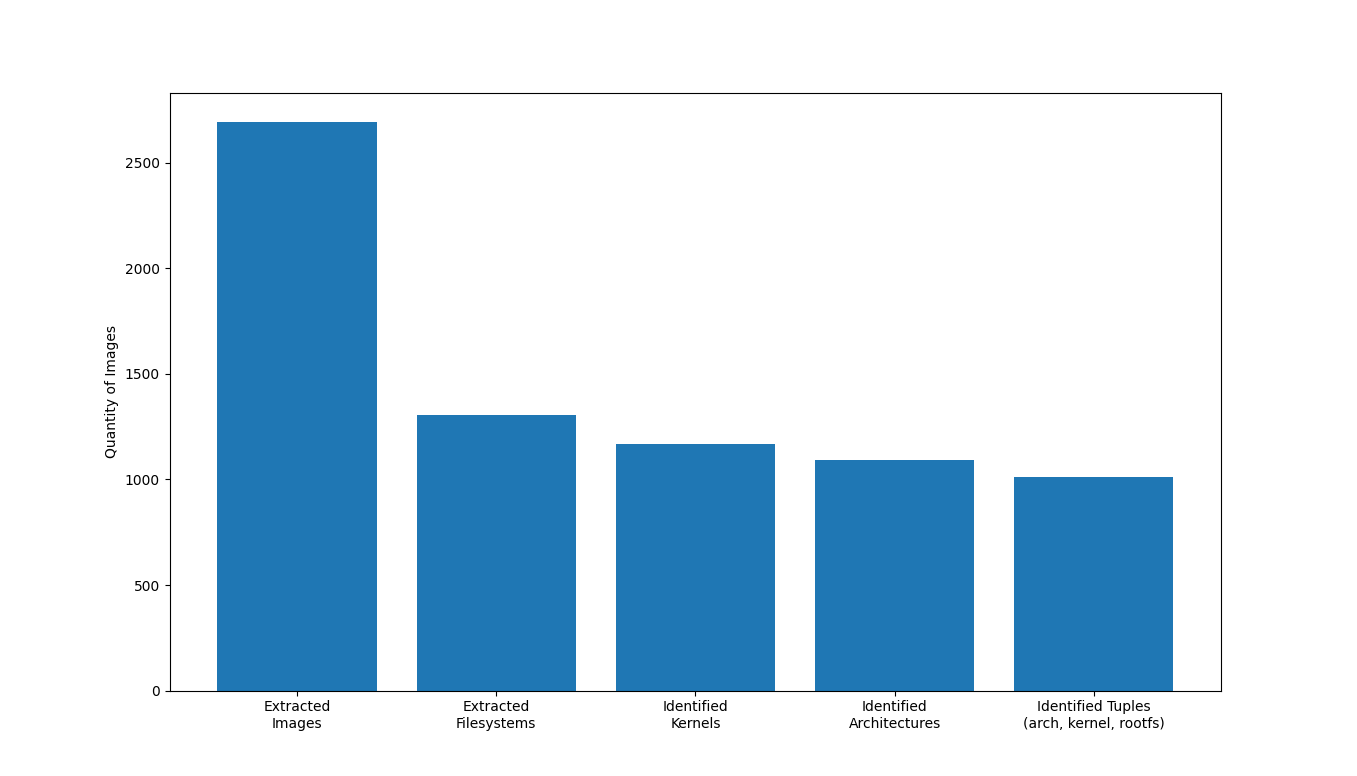
\includegraphics[width=0.90\textwidth]{figs/Funnel.png}
    \caption{Success funnel for firmware image extraction.}
    \label{fig:stats-funnel}
\end{figure}

It was also identified two issues in the extraction process. First, we observed incorrect identification in some kernel image media types (formerly known as MIME types) as a type on the extraction script denylist, which is easily corrected by excluding the identified type from the denylist. The second issue is related to the recursive extraction process. The limits in breadth and depth exploration allow the {\tt binwalk} tool to have functional performance, but in some cases, these limits were, in fact, responsible for the firmware extraction to be unsuccessful. Therefore, we believe in using a heuristic to select files with the most potential to hold firmware kernel or filesystem to be extracted next. This way, we can still have breadth and depth limits to maintain the extraction process feasibly, but it would also focus the extraction in more prominent files. Unfortunately, this approach of using heuristics, although idealized, was not yet implemented in our work.

Another enhancement we developed to the extraction process was the ability to extract additional kernel information. During kernel extraction, we scanned the kernel binary file for ASCII strings. From this search result, we then extract kernel banner (a string containing kernel version, compiler version used during kernel compilation, compilation date, and email of the developer who compiled the kernel) or identify, for instance, if the extracted system refers to an OpenWrt Linux. We store these additional pieces of information in a database. The database we implemented was also based on the database used by Firmadyne, but we had its schema altered to contain new columns to store the extra information we decided to collect.

% Falar das estatísticas; Colocar tabela com as estatísticas

\subsubsection{Statistics}

Regarding firmware extraction and feature identification, we collected some statistics that may help the following steps of this work in kernel compilation and firmware re-hosting. Table \ref{tab:arch-stats} shows the amount of firmware detected for each architecture identified. Tables \ref{tab:kernel-stats} and \ref{tab:kernel-family-stats} shows the five most common kernel versions and kernel families respectively. Also, Table \ref{tab:kernel-stats} shows the number of known CVEs for each kernel version. The number of known CVEs was extracted from the CVE Details \cite{cvedetails} database \footnote{For some kernel versions, the {\tt www.cvedetails.com} database contains repeated entries with a different number of known CVEs. The biggest number for each repeated version was chosen.}. For architectures and kernel families, we couldn't find a way to easily extract the number of known vulnerabilities from open sources of information.

\begin{table}[h]
\centering
\caption{Number of images identified for each found architecture}
\begin{tabular}{|c|c|}
\hline
\textbf{Architecture} & \textbf{Quantity of Images} \\ \hline
{\tt mipseb}                & 485                         \\ \hline
{\tt armel}                 & 336                         \\ \hline
{\tt mipsel}                & 249                         \\ \hline
{\tt mips64eb}              & 11                          \\ \hline
{\tt ppceb}                 & 10                          \\ \hline
{\tt intel64el}             & 1                           \\ \hline
\end{tabular}
\label{tab:arch-stats}
\end{table}

\begin{table}[h]
\centering
\caption{Five most common kernel versions found in extracted firmware images and number of known CVEs for each version.}
\begin{tabular}{|c|c|c|}
\hline
\textbf{Kernel Version} & \textbf{Quantity of Images} & \textbf{Number of known CVEs}  \\ \hline
2.6.31                  & 167           &    36 \\ \hline
2.6.36                  & 122           &    20 \\ \hline
3.3.8                   & 46            &    133 \\ \hline
3.14.77                 & 44            &    0 \\ \hline
2.6.22                  & 44            &    113 \\ \hline
\end{tabular}
\label{tab:kernel-stats}
\end{table}

\begin{table}[h]
\centering
\caption{Five most common kernel families found in extracted firmware images.}
\begin{tabular}{|c|c|}
\hline
\textbf{Kernel Family} & \textbf{Quantity of Images} \\ \hline
2.6                    & 484            \\ \hline
3.14                   & 63              \\ \hline
3.3                    & 46              \\ \hline
3.10                   & 38              \\ \hline
3.4                    & 33              \\ \hline
\end{tabular}
\label{tab:kernel-family-stats}
\end{table}

The information gathered in this phase is going to be used as a mean to select the first firmware files that are going to be re-hosted in future work as a mean to search for vulnerabilities.


\subsection{Kernel Cross-compilation \& Toolchain Building}

As shown by Table \ref{tab:kernel-family-stats}, kernel family 2.6 was the most commonly found amongst successfully extracted kernels. Therefore, we investigated the difficulties of cross-compiling a 2.6 Linux kernel. At first, we tried to cross-compile the kernel in a raw modern operating system. We chose Debian 10 (running with Linux kernel version 4.19) as the starting point for this experiment. In this environment, with {\tt gcc} version 8.3.0 as the compiler and using {\tt libc} version 2.28.10, it was not possible to compile the target kernel.

Then we downloaded an old version of the Debian operating system, with a release date similar to the 2.6 Linux kernel. We employ Debian 3.1r8 (kernel 2.4.27) for this experiment. Using this old operating system, with {\tt gcc} version 3.3.5 as the compiler and using {\tt libc} version 2.3.2, we had success in compiling the target kernel. Therefore, it highlights the impact the toolchain (compiler, binary utilities, and library versions) has on the kernel compiling process, and therefore, to achieve a way to automate kernel compiling, we also need a way to automate toolchain building. In this context, we adopted the {\tt crosstool-ng} tool. With this program, the user can define, between some pre-configured settings, specific versions for each tool inside the toolchain, and the program then tried to compile the desired toolchain.

Using {\tt crosstool-ng} we were then able to successfully compile a 2.6 Linux kernel inside a Debian 10 (modern operating system). However, when trying to cross-compile the target kernel for the {\tt MIPS} architecture (cross-compiling), we still faced issues that did not allow the kernel to compile successfully and require further investigation to build a working toolchain for this scenario.

\section{Conclusions}
\label{sec:conclusions}

We present SCREEN: {\bf S}craper, {\bf C}lustering, {\bf RE}-hosting, and {\bf E}xploitatio{\bf N} a framework to obtain, analyze small and home-office (SOHO), and exploit firmware from vendors' website.  Our solution allows a comprehensive view of this task, providing a concern-based division of responsibilities.  Moreover, we demonstrate this utilization by downloading $5265$ copies of the firmware from $5$ different vendors. Finally, we cross-compiled the most common kernel and reported future directions to increase the coverage of kernel-mode running artifacts.

From our obtained results so far, we could already improve in the state-of-the-art of identifying the kernel in about $19\%$ (from Firmadyne $983$ to $1169$) using our approach to find the kernel information inside files from the filesystem.  The Linux Kernel is the most adopted operating system, mainly in the family version {\tt 2.6}.  Precisely, the versions {\tt 2.6.31} and {\tt 2.6.36} correspond to the majority of the kernel-mode running software.  From the $1092$ identified firmware, MIPS is the preferred architecture (about $68\%$), followed by ARM (about $30\%$), PPC (about $1\%$), and Intel x86 with a single copy.  Other results include the extensive use of busybox to realize userland tools and the absence of sudoers users.  Finally, the cross-compiling tools are prominent to enable the re-hosting on a large scale; however, it requires a more considerable effort to reach its full potential.

As future work, we plan to acquire more firmware by adding other vendors and increase the information gathered from the local repository.  Also, improve the cross-compiling mechanisms and bring them to a level that allows automation; and then, develop metrics to measure the coverage in the re-hosting task. Finally, we aim to perform a large-scale re-hosting and vulnerability searching in the most prominent firmware images using the architecture illustrated by Figure \ref{fig:screen-approach} and will be able to investigate if a large-scale attack against home network routers could be feasible and in this case, how it could be avoided.


\section*{Acknowledgements}

This work was supported in part by ITA's Programa de Pós-graduação em Aplicações Operacionais (ITA/PPGAO).

\bibliographystyle{sbc}
\bibliography{referencias}

\end{document}
